\documentclass[10pt,a4paper]{article}
%standard symbols
\usepackage{amssymb, amsmath, esint, mathrsfs, tipa}
%charts and tables
\usepackage{array, enumitem}
%graphics
\usepackage{graphicx}
%packages for float
\usepackage{wrapfig, placeins, float}
%specialized tools
\usepackage[americanvoltages,RPvoltages]{circuitikz}
%geometry
\usepackage[left=1.0cm, right=1.0cm, top=2.5cm]{geometry}
%code
\usepackage{listings}
%links
\usepackage{hyperref}

\setlength{\textfloatsep}{5pt plus 2pt minus 2pt}
\setlength{\floatsep}{5pt plus 2pt minus 2pt}

\begin{document}

%\tableofcontents

\section{Introduction}

These are a collection of personal notes on the ODMB, an circuit board used by the CMS CSC detectors.

\section{ODMB Firmware}

\subsection{Top Level}

The current ODMB is largely split into two pieces The first is ODMB VME (MBV), which executes slow control such as sending commands to DCFEB or LVMB and changing ODMB settings. The second is ODMB CTRL (MBC), which executes fast control needed during data taking.

%clock generation and qpll interface
The 160MHz and 40MHz clocks are produced by the qpll. The \texttt{qpll\_reset} and \texttt{qpll\_autorestart} signals are held at `1'. The faster clocks (10 MHz, and 5 MHz) are generated by a clock manager (MMCM) ip core from the 40 MHz clock. The slightly slower clocks (2.5 MHz, 5 MHz, 1.25 MHz, 0.625 MHz) are generated by dividing the 5 MHz clock with D flops. Finally, the very slow clocks (10 kHz and 1 kHz) are generated in a process with a counter.

%VME interface
The VME interface consists of several signals, which go to the IC's on the ODMB that ultimately interface with the VME backplane. These signals are summarized in table \ref{tab:vmeinterface}. Inside the ODMB, most of these signals are sent to the \texttt{COMMAND\_MODULE} module in ODMB VME, which decodes the VME commands and send appropriate signals such as \texttt{STROBE}, \texttt{DEVICE}, and \texttt{COMMAND} to the ODMB VME devices. 

For more on VME protocol, see \href{http://www.interfacebus.com/Design_Connector_VME.html}{VME Reference}.

\begin{table}[H]
\begin{tabular}{|l|l|} \hline
Port& Description\\ \hline
\texttt{vme\_data}& VME data IO line, IOBUF controlled by \texttt{vme\_tovme (bar)}\\ \hline
\texttt{vme\_addr}& address from VME, given to \texttt{COMMAND\_MODULE}\\ \hline
\texttt{vme\_am}& address modifier from VME, given to \texttt{COMMAND\_MODULE}\\ \hline
\texttt{vme\_gap}& geographical address parity from VME, given to \texttt{COMMAND\_MODULE}\\ \hline
\texttt{vme\_ga}& geographical address from VME, given to \texttt{COMMAND\_MODULE}\\ \hline
\texttt{vme\_as\_b}& address strobe (bar) from VME, given to \texttt{COMMAND\_MODULE} and \texttt{VMECONFREGS}\\ \hline
\texttt{vme\_ds\_b}& data strobe (bar) from VME, given to \texttt{COMMAND\_MODULE}\\ \hline
\texttt{vme\_sysfail\_b}& sysfail (bar) signal from VME, given to \texttt{COMMAND\_MODULE}\\ \hline
\texttt{vme\_sysfail\_out}& sysfail signal to VME, tied to `0'\\ \hline
\texttt{vme\_berr\_b}& error (bar) signal from VME, given to \texttt{COMMAND\_MODULE}\\ \hline
\texttt{vme\_berr\_out}& error signal to VME, tied to `0'\\ \hline
\texttt{vme\_iack\_b}& instruction acknowledge from VME, given to \texttt{COMMAND\_MODULE}\\ \hline
\texttt{vme\_lword\_b}& load word signal from VME, given to \texttt{COMMAND\_MODULE}\\ \hline
\texttt{vme\_write\_b}& write (bar) signal from VME, given to each device in \texttt{ODMB VME}\\ \hline
\texttt{vme\_dtack\_v6\_b}& data acknowledge (bar) signal to VME, low when any \\
                 & device from ODMB VME issues a dtack\\ \hline
\texttt{vme\_tovme}& output signal controlling direction of \texttt{vme\_data}. not \\
          & \texttt{tovme\_b} from \texttt{COMMAND\_MODULE}\\ \hline
\texttt{vme\_doe\_b}& VME output enable (bar) signal from \texttt{COMMAND\_MODULE}\\ \hline
\end{tabular}
\caption{Signals in VME interface}
\label{tab:vmeinterface}
\end{table}

\subsection{DCFEB JTAG and INITJAG}

The DCFEB JTAG device (cfebjtag.vhd) is the first device in the ODMB VME interface. This module is used to communicate with (x)(D)CFEBs via JTAG protocol (via the PPIB skew clear cables). The signals connecting to this interface are listed in table \ref{tab:cfebjtaginterface}.

\begin{table}[H]
\begin{tabular}{|l|l|} \hline
Port& Description\\ \hline
\texttt{FASTCLK}& 40MHz clock from top level\\ \hline
\texttt{SLOWCLK}& 2.5MHz clock from top level. Called \texttt{clk\_s1} in odmb\_vme.vhd and top level and said \\
       &to be 10 MHz/0.625 MHz in incorrect comments\\ \hline
\texttt{RST}& Reset signal.\\ \hline
\texttt{DEVICE}& Signal to accept/ignore incoming commands/strobes. Should be connected to DEVICE(1) \\
      & output from \texttt{COMMAND\_MODULE}, which decodes VME commands- will be 1 for \\
			& VME commands 1XXX.\\ \hline 
\texttt{STROBE}& Signal that initiates command execution; generated by \texttt{COMMAND\_MODULE} \\
      & from VME strobe signals\\ \hline
\texttt{COMMAND}& Important bits of VME command (append ``00'' to end for full command)\\ \hline
\texttt{WRITER}& Unused, connected from \texttt{VME\_WRITE\_B}\\ \hline
\texttt{INDATA}& input directly from \texttt{VME\_DATA} line (through IOBUF)\\ \hline
\texttt{OUTDATA}& output multiplexed to \texttt{VME\_DATA} line (through IOBUF)\\ \hline
\texttt{DTACK}& acknowledge receipt of VME commands, OR'd with DTACKs from other devices \\
     & and sent back to VME. Active high\\ \hline
\texttt{INITJTAGS}& signal that resets module and sends signals to reset CFEB JTAG \\
         & state machine, generated when DONE received from (x)(D)CFEBs\\ \hline
\texttt{TCK}& JTAG output to (x)(D)CFEB, one per (x)(D)CFEB\\ \hline
\texttt{TDI}& JTAG output to (x)(D)CFEB, common to all (x)(D)CFEBs\\ \hline
\texttt{TMS}& JTAG output to (x)(D)CFEB, common to all (x)(D)CFEBs\\ \hline
\texttt{FEBTDO}& JTAG input from (x)(D)CFEB, one per (x)(D)CFEBs\\ \hline
\texttt{LED}& DEBUG output\\ \hline
\texttt{DIAGOUT}& DEBUG output\\ \hline
\texttt{CSP\_LVMB\_LA\_CTRL}& Unused\\ \hline
\end{tabular}
\caption{Signals in CFEBJTAG device}
\label{tab:cfebjtaginterface}
\end{table}

%on TCK generation
When a STROBE signal is received and there is an appropriate VME command, a LOAD signal is generated, which then generates a BUSY signal. The BUSY signal then causes the global TCK clock to run. It has been observed that sometimes, a `ghost strobe' signal is received, which causes TCK to run with TMS/TDI set to a constant 0. This may result in strange commands being sent to the (x)(D)CFEBs. The appearance of these ghost strobes seem to change with unrelated changes to firmware, indicating a race condition or something similar. 

%on TMS generation
The TMS signals are generated by loops of sequentially connected D flops. By using FDC(E) and FDP(E) flops, certain sequences of 1's and 0's are achieved in order to control the JTAG state machine. The FD flops from the \texttt{Latches\_Flipflops} package are found not to work on the KCU105 evaluation board and were replaced with the equivalent UNISIM components. Furthermore, the CB4CE and SR16LCE functions from the \texttt{Latches\_Flipflops} package did not defaultly work on the KCU105 evaluation board, and their implementation was slightly tweaked to nest conditions rather than AND'ing them. It is unclear why this changes behavior.

%on DCFEB_DONE FSM in top level
The \texttt{INITJTAG} signal is generated after receiving DONE from the (x)(D)CFEBs. The signal \texttt{pon\_rst\_reg} is initialized to a particular value when \texttt{PLL\_LOCK} is on (when ODMB is reset) and after a few clock cycles, \texttt{pon\_reset} becomes '1', which sets the FSM \texttt{done\_current\_state} to \texttt{DONE\_LOW}. When the \texttt{DONE} for an (x)(D)CFEB becomes `1', the \texttt{done\_current\_state} is set to \texttt{DONE\_COUNTING}, which generates \texttt{dcfeb\_done\_pulse} before setting the FSM to \texttt{DONE\_IDLE}. All the \texttt{dcfeb\_done\_pulse}'s are OR'd together and converted to a pulse to generate \texttt{INITJTAG}. Perhaps this logic could be moved from the top level to inside of cfebjtag.vhd. Note that the FSM counter runs on the 10 kHz clock, which is just generated in a process somewhere and not BUFG'd. 

\subsection{Command Module}

The command module (command.vhd) is a helper device in the ODMB VME interface responsible for decoding the signals received from the VME backplane. The signals connecting to this interface are listed in table \ref{tab:commandinterface}.

\begin{table}[H]
\begin{tabular}{|l|l|} \hline
Port& Description\\ \hline
\texttt{FASTCLK}& 40MHz clock from top level\\ \hline
\texttt{SLOWCLK}& 2.5MHz clock from top level\\ \hline
\texttt{GA}& VME geographical address from \texttt{VME\_GA} and \texttt{VME\_GAP} (\texttt{GA(5)} should be \texttt{VME\_GAP})\\ \hline
\texttt{ADR}& VME address from \texttt{VME\_ADDR}\\ \hline
\texttt{AM}& VME address modifier from \texttt{VME\_AM}\\ \hline
\texttt{AS}& VME address strobe (bar) from \texttt{VME\_AS\_B}\\ \hline
\texttt{DS0}& Lower bit of VME data strobe (bar) from \texttt{VME\_DS\_B(0)}\\ \hline
\texttt{DS1}& Upper bit of VME data strobe (bar) from \texttt{VME\_DS\_B(1)}\\ \hline
\texttt{LWORD}& VME load word (bar) from \texttt{VME\_LWORD\_B}\\ \hline
\texttt{WRITER}& VME write (bar) signal from \texttt{VME\_WRITE\_B}\\ \hline
\texttt{IACK}& VME interrupt acknowledge (bar) from \texttt{VME\_IACK\_B}\\ \hline
\texttt{BERR}& VME error (bar) signal from \texttt{VME\_BERR\_B}\\ \hline
\texttt{SYSFAIL}& VME SYSFAIL (bar) signal from \texttt{VME\_SYSFAIL\_B}\\ \hline
\texttt{TOVME\_B}& signal controlling \texttt{VME\_DATA} IOBUF at top level and output as (barred) \texttt{VME\_TOVME}\\ \hline
\texttt{DOE\_B}& VME output enable (bar) output as \texttt{VME\_DOE\_B}\\ \hline
\texttt{DEVICE}& each of 10 bits indicates to ODMB VME device if it is selected\\ \hline
\texttt{STROBE}& signal sent to ODMB VME devices to indicate command ready\\ \hline
\texttt{COMMAND}& decoded VME command sent to each ODMB VME device\\ \hline
\texttt{ADRS}& used to multiplex \texttt{VME\_DATA\_OUT} from the various devices\\ \hline
\texttt{DIAGOUT}& for debugging\\ \hline
\texttt{LED}& for debugging\\ \hline
\end{tabular}
\caption{Signals in command module device}
\label{tab:commandinterface}
\end{table}

This device loads \texttt{AM} into \texttt{AMS} when \texttt{AS} is '1'. When \texttt{DS} are both low, \texttt{AMS} is appropriate, and other signals are okay, a strobe is generated.

\subsection{VME Simulation}

The VME simulation is described by the state machine in figure \ref{fig:vmestatemachine}. Although the time-out functionality works in simulation, it works inconsistently on the KCU105 evaluation board. 

\begin{figure}[H]
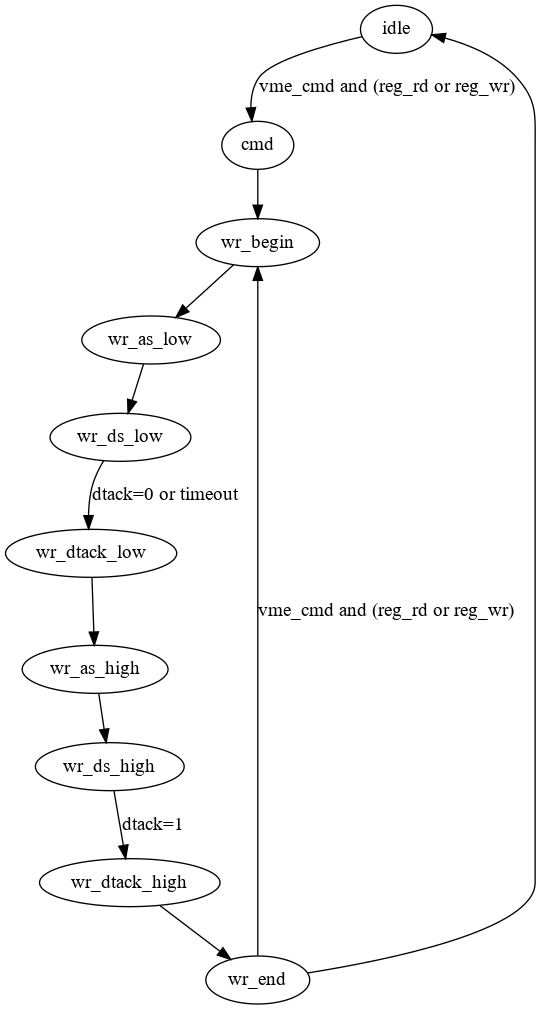
\includegraphics[width= 0.4 \textwidth]{figures/vmestates.png}
\caption{Simulated VME state machine}
\label{fig:vmestatemachine}
\end{figure}

%\bibliography{writeup}
%\bibliographystyle{plain}

\end{document}
